% intro.tex

%In this chapter we will present our findings and evaluate what impact the added features have on a working node.
In this chapter we will present the data we have collected from our measurements and how they were taken.

While management and monitoring can be both useful and convenient, it does introduce overhead. This overhead should not have a significant impact on system performance, others citing as low as 1-2\% impact as tolerable.

Here we will verify the impact of our work on the overall throughput and performance of the software under different workloads. We will look at requests processed per second and response time distribution under typical usage patterns and some edge cases. 

We will first look at single node performance, with and without our modifications.
Next we will try verifying that performance scaling is intact. For Voldemort, near linear scaling of throughput is expected when adding worker nodes to the cluster.
Lastly we will look at performance during a automatically triggered rebalance under load.

\section{The tests}
All tests are run on a clean cluster instance, with a warm up period loading data into the database. All tests are run three times, with the average score used.

Test0:

100\% read ?
100\% read no mod ?

99\% 1\% read/update ? read/write?
99\% 1\% read/update ? read/write? no mod

1\%/99\% read/write ?
1\%/99\% read/write ? no mod

linear scaling:
100\% read ? 2 nodes
100\% read no mod ? 2 nodes

99\% 1\% read/update ? read/write? 2 nodes
99\% 1\% read/update ? read/write? no mod | 2 nodes

These are the most realistic workloads for Voldemort, as a high volume read only service and about 98-99\% read to write/update.

rebalance:
Just monitor request rate during a rebalance.
Remember to somewhat record size of data set.

\begin{center}
\begin{table}[h]
	\begin{tabular}{|c|c|c|l|}
		\multicolumn{1}{c}{Test case} & 
		\multicolumn{1}{c}{read \%} & 
		\multicolumn{1}{c}{write \%} & 
		\multicolumn{1}{c}{state} \\
		\hline

		TC0 & 100 & 0 & no mod \\
		TC1 & 100 & 0 & mod \\
		TC2 & 99 & 1 & no mod \\
		TC3 & 99 & 1 & mod \\
		TC4 & 1 & 99 & no mod \\
		TC5 & 1 & 99 & mod \\

		\hline
	\end{tabular}
	\caption{Test case setup. No mod/mod is shorthand for no modification and modification, meaning whether we will be using original or our source code for this test.}
	\label{tbl:testcases}
\end{table}
\end{center}

Findings:

Network is of the utmost importance.

Performance seem very consistent.

% figures.tex


\begin{figure}[h]
    \centering
    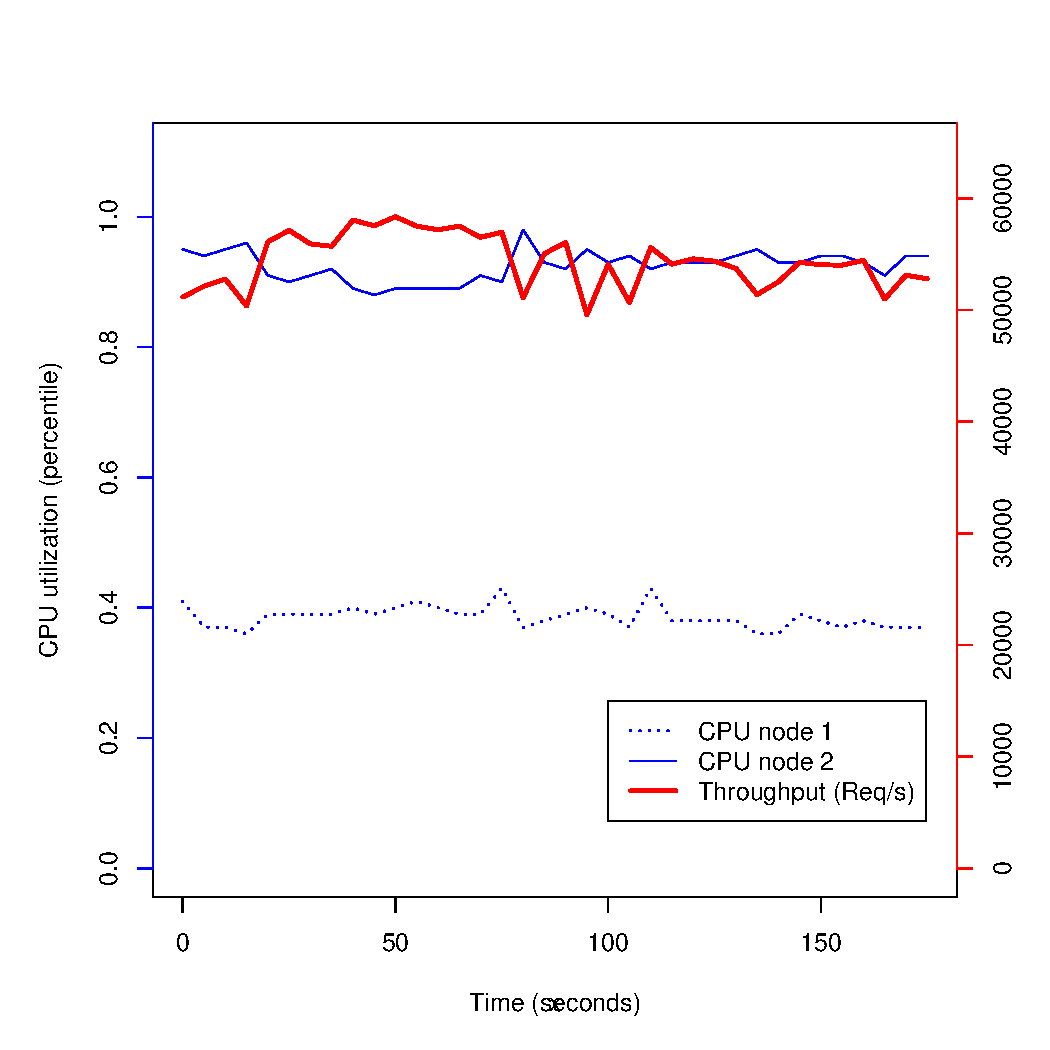
\includegraphics[width=1.2\textwidth]{results/baseline_plot}
    \caption{Baseline}
    \label{fig:baseline}
\end{figure}

\begin{figure}[h]
    \centering
    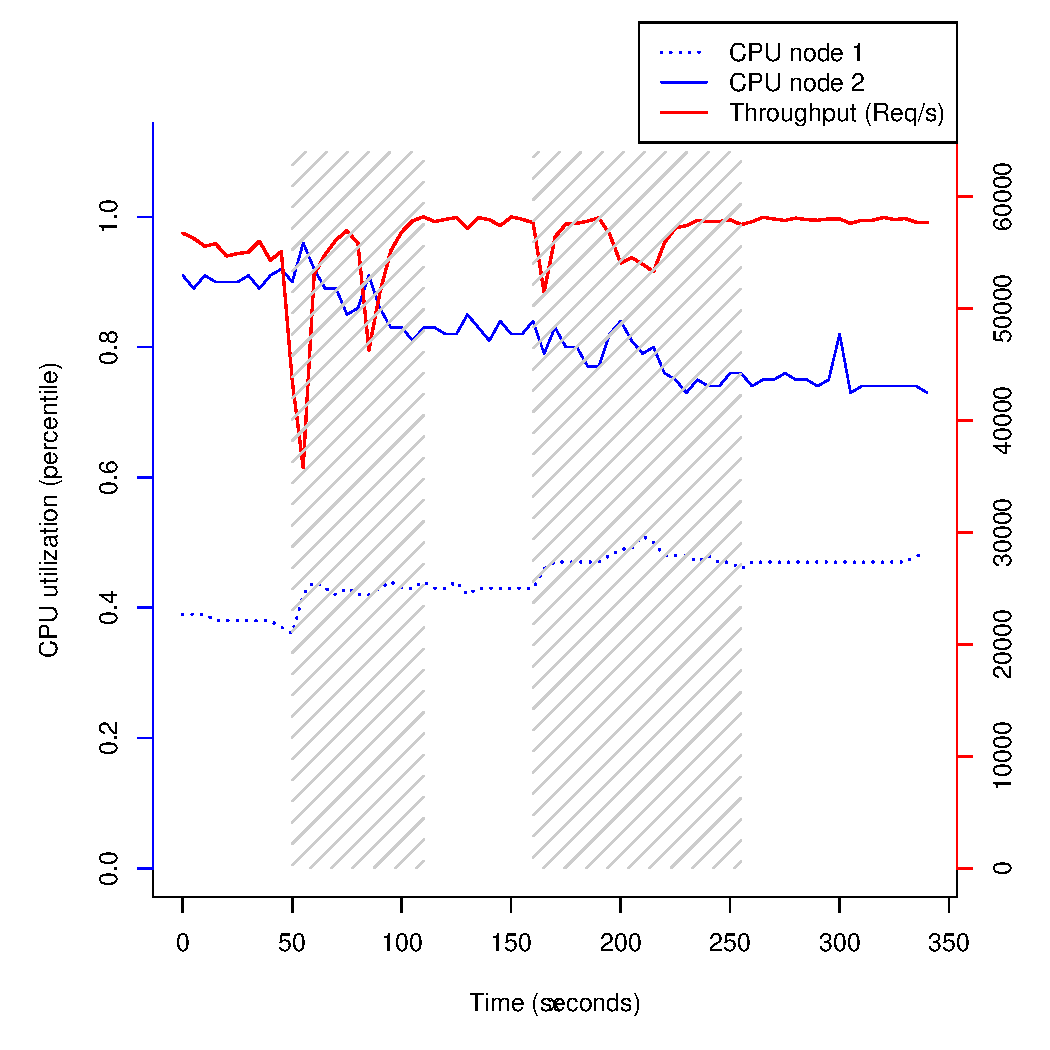
\includegraphics[width=1.2\textwidth]{results/adaptive_plot}
    \caption{Moving of 3 partitions from a struggling node (Node )}
    \label{fig:adaptive}
\end{figure}

